\documentclass[a11paper, 11pt]{article}

\usepackage{document}
\usepackage{titlepage}
% Allows to include standalone files as figures
\usepackage{graphicx}
\usepackage{float}
\usepackage{pgf-umlcd}
\usepackage[T1]{fontenc}
\usepackage[french]{babel}
\usepackage{csquotes}

% \addbibresource{bibliography.bib}
% \nofiles

% \institution{Université de Sherbrooke}
% \faculty{Faculté de génie}
% \department{Département de génie électrique et de génie informatique}
\title{Rapport d'APP}
\classnb{GIF350}
\class{APP1 -- Modèles de conception}
\author{
  \addtolength{\tabcolsep}{-0.4em}
  \begin{tabular}{rcl} % Ajouter des auteurs au besoin
  Samuel Bilodeau  & -- & BILS2704 \\ % TODO: demander le CIP
  Benjamin Chausse & -- & CHAB1704 \\
  \end{tabular}
}
\teacher{Domingo Palao Munoz}
% \location{Sherbrooke}
% \date{\today}

\begin{document}
\maketitle
\newpage
\tableofcontents
\newpage
\section{Diagrammes de classes}

\begin{figure}[H]
  \centering
  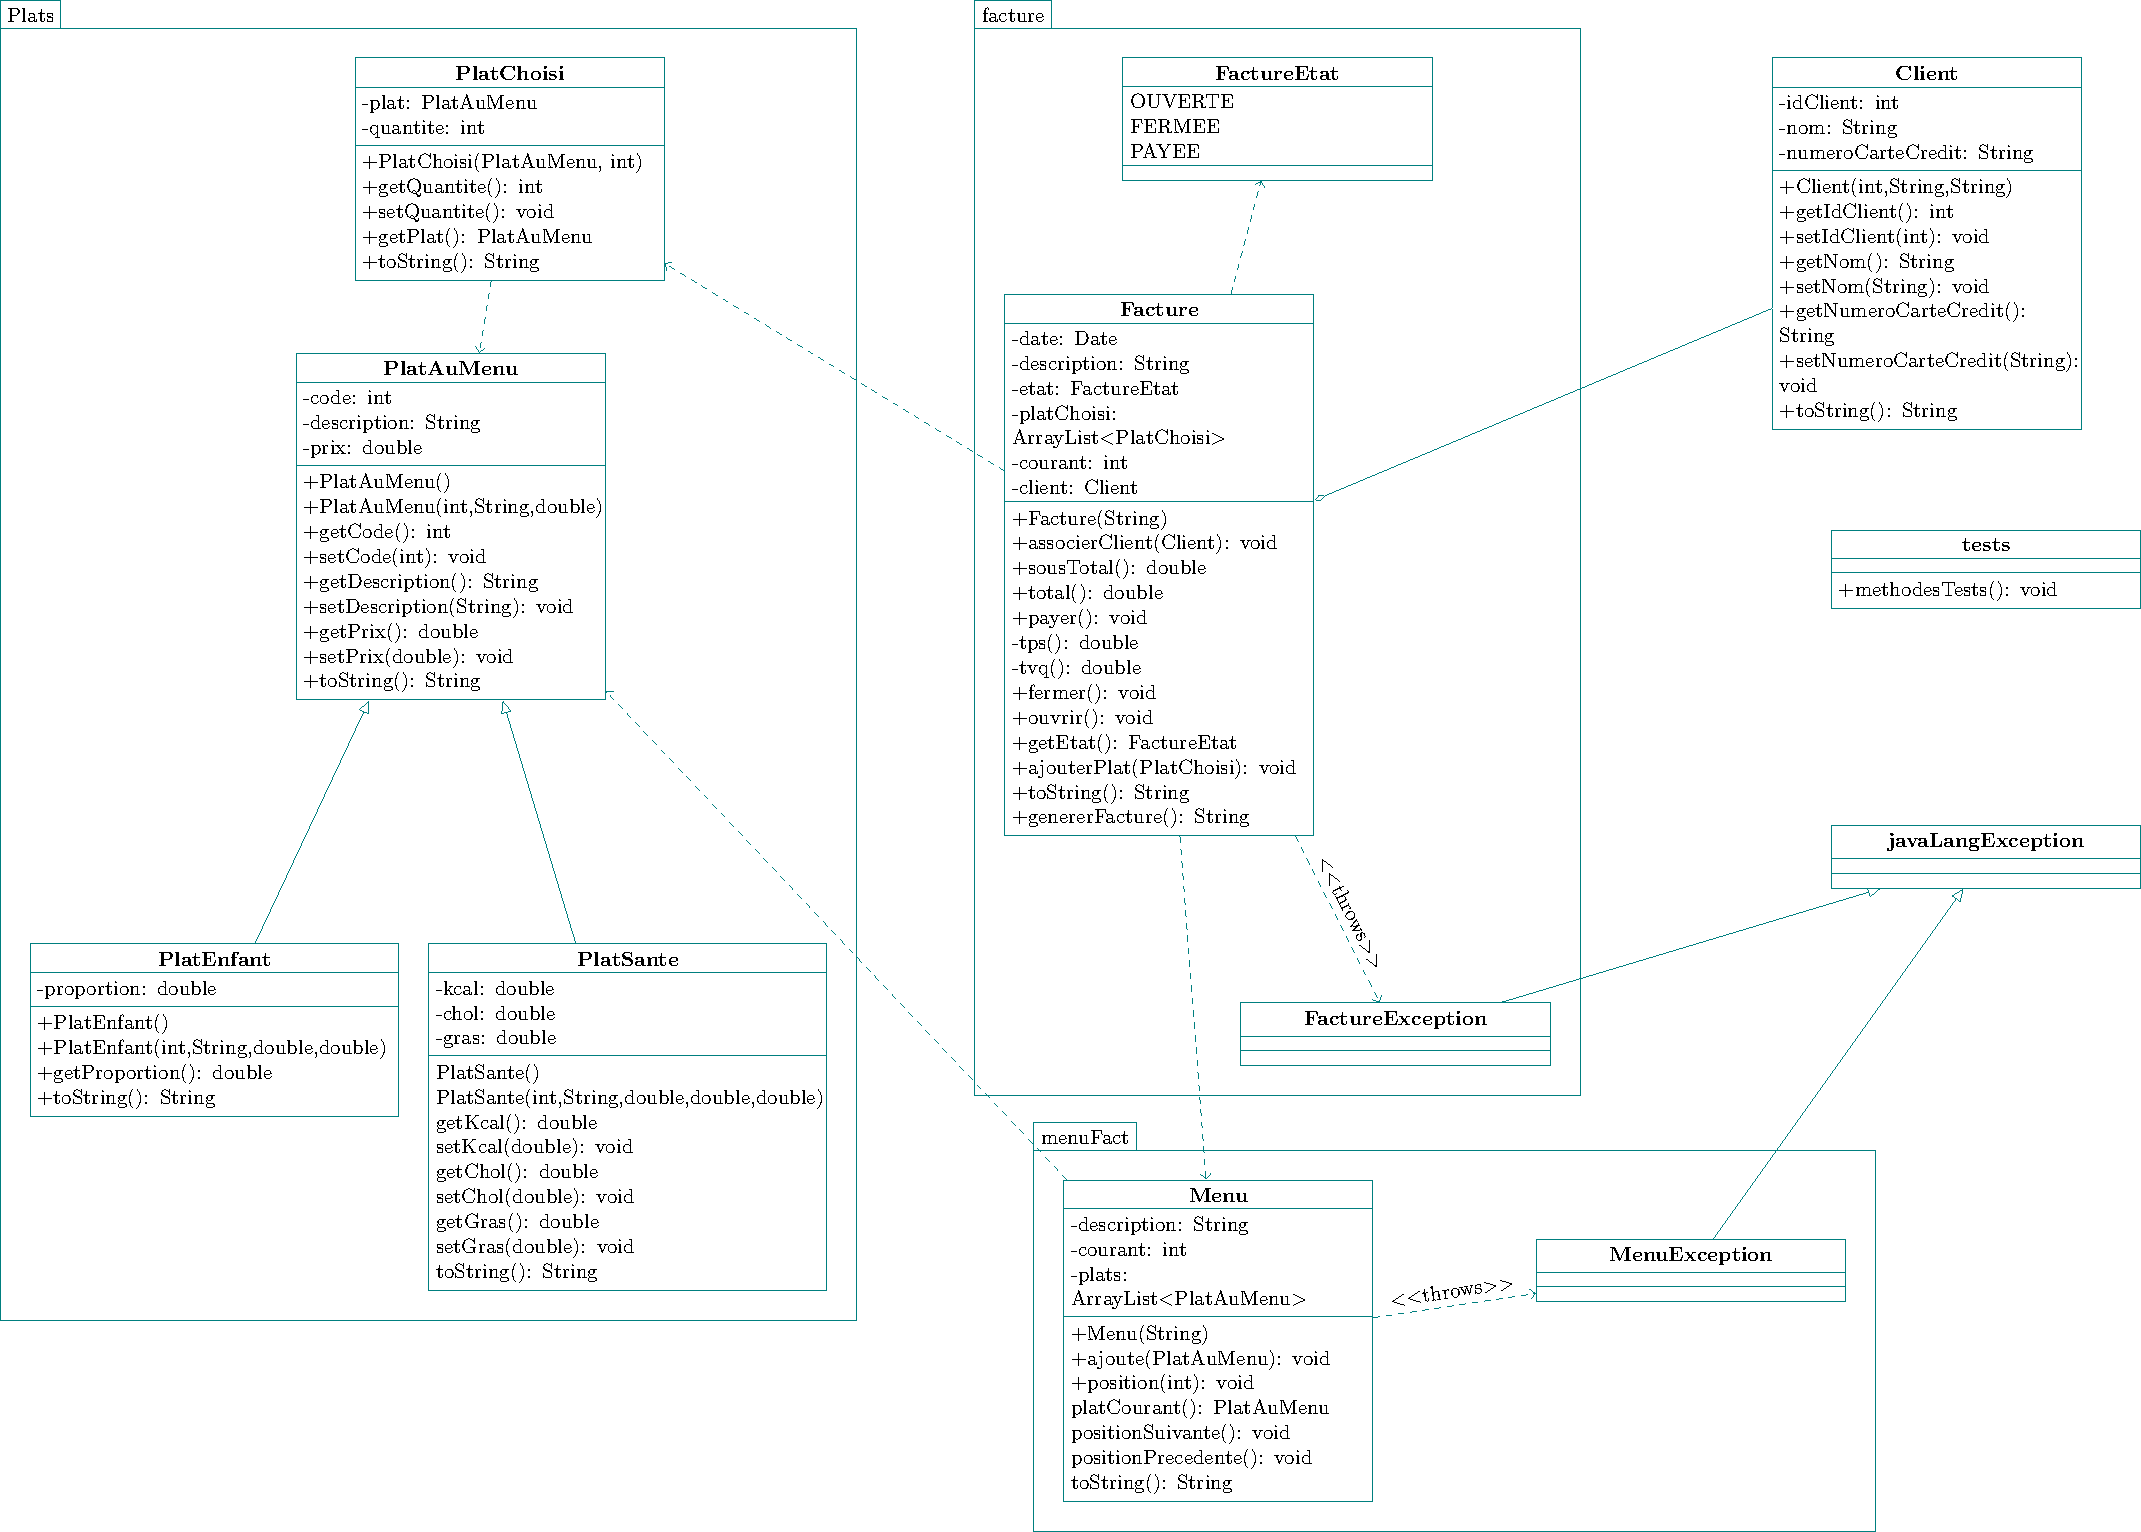
\includegraphics[width=\textwidth]{uml/uml.pdf}
  \caption{Diagramme de classes}
  \label{fig:uml}
\end{figure}


% \newpage
% \printbibliography[heading=bibintoc]
\end{document}
